\documentclass[a4paper,12pt]{article}
\usepackage[top = 2.5cm, bottom = 2.5cm, left = 2.5cm, right = 2.5cm]{geometry}
\usepackage[T1]{fontenc}
\usepackage[utf8]{inputenc}
\usepackage{multirow} 
\usepackage{booktabs} 
\usepackage{graphicx}
\usepackage[spanish]{babel}
\usepackage{setspace}
\setlength{\parindent}{0in}
\usepackage{float}
\usepackage{fancyhdr}
\usepackage{amsmath}
\usepackage{amssymb}
\usepackage{amsthm}
\usepackage[numbers]{natbib}
\newcommand\Mycite[1]{%
	\citeauthor{#1}~[\citeyear{#1}]}
\usepackage{graphicx}
\usepackage{subcaption}
\usepackage{booktabs}
\usepackage{etoolbox}
\usepackage{minibox}
\usepackage{hyperref}
\usepackage{xcolor}
\usepackage[skins]{tcolorbox}
%---------------------------

\newtcolorbox{cajita}[1][]{
	 #1
}

\newenvironment{sol}
{\renewcommand\qedsymbol{$\square$}\begin{proof}[\textbf{Solución.}]}
	{\end{proof}}

\newenvironment{dem}
{\renewcommand\qedsymbol{$\blacksquare$}\begin{proof}[\textbf{Demostración.}]}
	{\end{proof}}

\newtheorem{problema}{Problema}
\newtheorem{definicion}{Definición}
\newtheorem{ejemplo}{Ejemplo}
\newtheorem{teorema}{Teorema}
\newtheorem{corolario}{Corolario}[teorema]
\newtheorem{lema}[teorema]{Lema}
\newtheorem{prop}{Proposición}
\newtheorem*{nota}{\textbf{NOTA}}
\renewcommand\qedsymbol{$\blacksquare$}
\usepackage{svg}
\usepackage{tikz}
\usepackage[framemethod=default]{mdframed}
\global\mdfdefinestyle{exampledefault}{%
linecolor=lightgray,linewidth=1pt,%
leftmargin=1cm,rightmargin=1cm,
}




\newenvironment{noter}[1]{%
\mdfsetup{%
frametitle={\tikz\node[fill=white,rectangle,inner sep=0pt,outer sep=0pt]{#1};},
frametitleaboveskip=-0.5\ht\strutbox,
frametitlealignment=\raggedright
}%
\begin{mdframed}[style=exampledefault]
}{\end{mdframed}}
\newcommand{\linea}{\noindent\rule{\textwidth}{3pt}}
\newcommand{\linita}{\noindent\rule{\textwidth}{1pt}}

\AtBeginEnvironment{align}{\setcounter{equation}{0}}
\pagestyle{fancy}

\fancyhf{}









%----------------------------------------------------------
\lhead{\footnotesize Álgebra Moderna}
\rhead{\footnotesize  Rudik Roberto Rompich}
\cfoot{\footnotesize \thepage}


%--------------------------

\begin{document}
 \thispagestyle{empty} 
    \begin{tabular}{p{15.5cm}}
    \begin{tabbing}
    \textbf{Universidad del Valle de Guatemala} \\
    Departamento de Matemática\\
    Licenciatura en Matemática Aplicada\\\\
   \textbf{Estudiante:} Rudik Roberto Rompich\\
   \textbf{Correo:}  \href{mailto:rom19857@uvg.edu.gt}{rom19857@uvg.edu.gt}\\
   \textbf{Carné:} 19857
    \end{tabbing}
    \begin{center}
        MM2035 - Álgebra Moderna - Catedrático: Ricardo Barrientos\\
        \today
    \end{center}\\
    \hline
    \\
    \end{tabular} 
    \vspace*{0.3cm} 
    \begin{center} 
    {\Large \bf  Tarea 13
} 
        \vspace{2mm}
    \end{center}
    \vspace{0.4cm}
%--------------------------

\section{Con la información del caso, basado en los Exhibits 1 y 2, construyan el Flujo de Caja de los mismos periodos que los otros estados financieros.}

\begin{figure}[H]
    \centering
    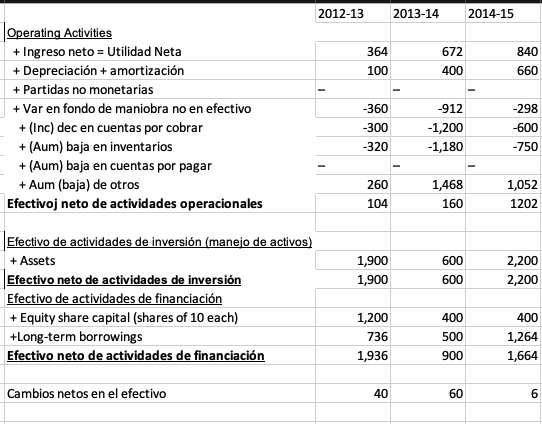
\includegraphics[scale=0.5]{Problemas/1}
    \caption{Flujo de efectivo}
\end{figure}

\section{Ingresen en Excel la información de los estados financieros y analicen la tendencia de las cuentas macro más importantes.}

\begin{figure}[H]
    \centering
    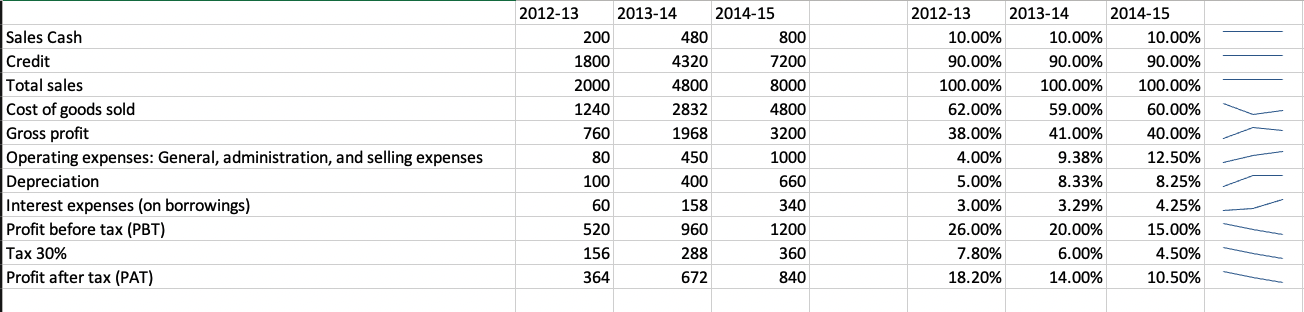
\includegraphics[scale=0.3]{Problemas/2}
    \caption{Análisis vertical}
\end{figure}

Al analizar la tendencia del flujo de efectivo para el estado de resultados, puedo notamos que las ventas totales han sido constantes. Por otra parte, es preocupante la tendencia bajista de el costo de los bienes vendidas y las ganancias en general. Por otra parte, también es de notar que los costos operativos la depreciación y los interés han ido en subida. En general, el análisis muestra que la empresa no está tan bien. 


\section{Calculen y analicen todas las razones financieras (las mismas que la Exhibit 3) para la empresa analizada.}


\begin{figure}[H]
    \centering
    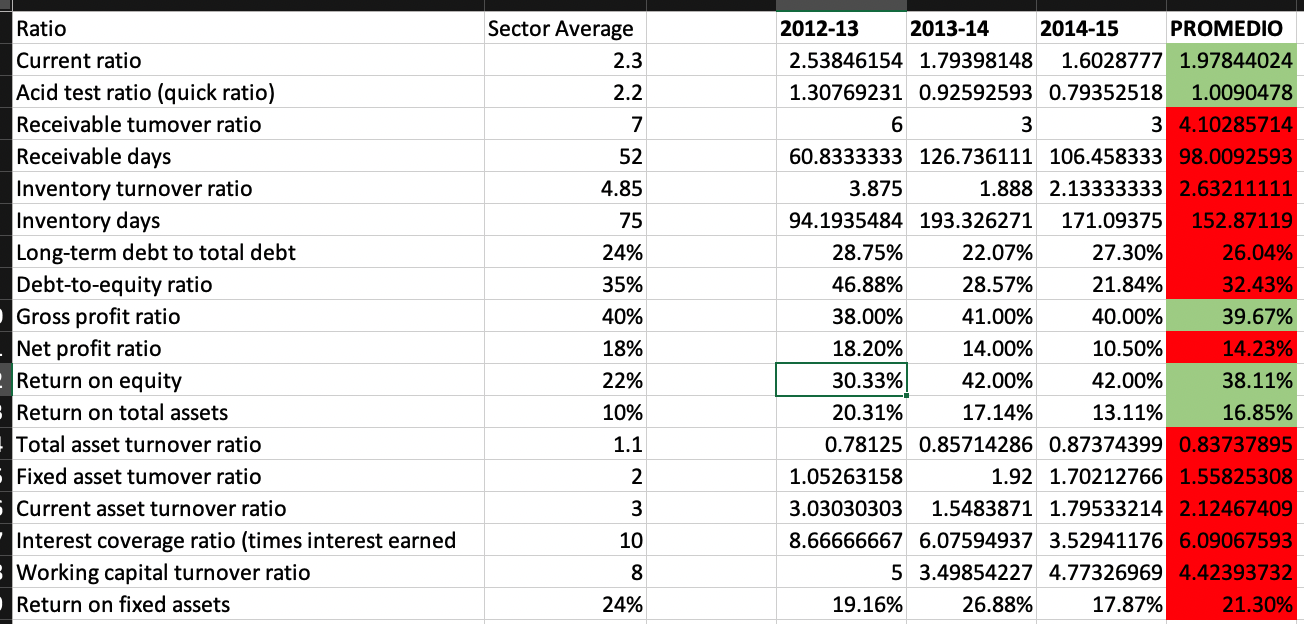
\includegraphics[scale=0.3]{Problemas/3}
\end{figure}

En general, pensaría que los indicadores son bastante claros, la empresa no le está yendo muy bien. Podemos notar que que el retorno en la equidad es bastante más alto al promedio del sector, igual que la proporción de ganancia. También la razón corriente y la prueba ácida muestra resultados que indican que la empresa tiene liquidez. Sin embargo, las demás razones están por debajo de lo esperado, lo que indica que la empresa en general no está muy bien. 

\section{Basándose en las razones financieras calculadas, y las de la industria, ¿darían el préstamo si fueran los encargados de tomar la decisión?}

No, no la daría. La empresa tiene muchos indicadores negativos y el análisis vertical es desalentador. El futuro de la empresa pareciera no ser el mejor. 


%---------------------------
%\bibliographystyle{apa}
%\bibliography{referencias.bib}

\end{document}